\section[Xbase]{Implementation in Xbase}

\begin{frame}
  \frametitle{Implementation in Xbase}
  \tableofcontents[currentsection]
\end{frame}
  
\begin{frame}[fragile,allowframebreaks]
  \frametitle{Implementation in Xbase}
  \begin{itemize}
    \item Attributes of entities refer to Java elements
    \item Infer Java type for Entities and Forms with
    \emph{JvmModelInferrer}
  \end{itemize}
  
  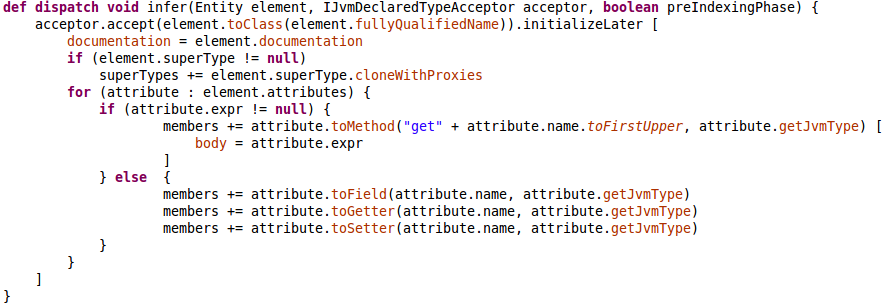
\includegraphics[width=\linewidth]{img/xbase-infer.png}  
 
  \begin{verbatim}
    	def dispatch void infer(Entity element, IJvmDeclaredTypeAcceptor acceptor, boolean preIndexingPhase) {
   		acceptor.accept(element.toClass(element.fullyQualifiedName)).initializeLater [
			documentation = element.documentation
			if (element.superType != null)
				superTypes += element.superType.cloneWithProxies
		    for (attribute : element.attributes) {
		    	if (attribute.expr != null) {
						members += attribute.toMethod("get" + attribute.name.toFirstUpper, attribute.getJvmType) [
			        		body = attribute.expr
		        		]
		        } else  {
		            	members += attribute.toField(attribute.name, attribute.getJvmType)
			            members += attribute.toGetter(attribute.name, attribute.getJvmType)
			            members += attribute.toSetter(attribute.name, attribute.getJvmType)
		        }
		    }
   		]
   	}

 	def dispatch void infer(Form form, IJvmDeclaredTypeAcceptor acceptor, boolean preIndexingPhase) {
   		acceptor.accept(form.toClass(form.fullyQualifiedName)).initializeLater [
			documentation = form.documentation
		    for (widget: form.widgets) {
		    	if (widget.validate != null && widget.attr != null) {
		    		members += widget.toMethod('validate'+widget.attr.name.toFirstUpper, form.newTypeRef(Boolean::TYPE)) [
		    			parameters += widget.toParameter("it", form.entity.getJvmType)
		    			parameters += widget.toParameter("widgetcontent", widget.attr.getJvmType)
		    			body = widget.validate
		    		]
		    	}
		    }   		 	
   		]
   	}
  \end{verbatim}
  
\end{frame}